\subsection{Strassen's vs IJK-Algorithm:}

First versus of {\bfseries\itshape Strassen's Algorithm} against {\bfseries\itshape IJK-Algorithm}. The program will plot the {\bfseries\itshape time} that both algorithm's takes to make the product of matrices of size {\itshape  n = $2^{8}$}. \hfill \break

{\bfseries\itshape\color{carmine}{Observation:}} {\itshape\color{carmine}{Both matrices A and B are to big to put a screen-shot of the console output, same for the resulting matrix. In compensation we will put the algorithms parameters in the console output for plotting both complexities.}} \hfill \break

\begin{figure}[H]
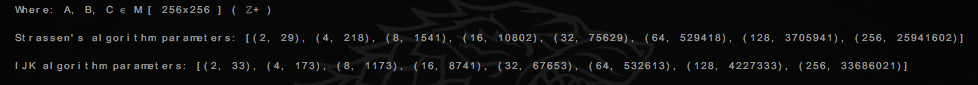
\includegraphics[width = 16.5cm, height = 1.5cm]{v1.png}
\centering \linebreak \linebreak Figure 4.2.0: Parameters of Strassen's and IJK algorithms for matrices of size n = $2^{8}$.
\end{figure} 

\begin{figure}[H]
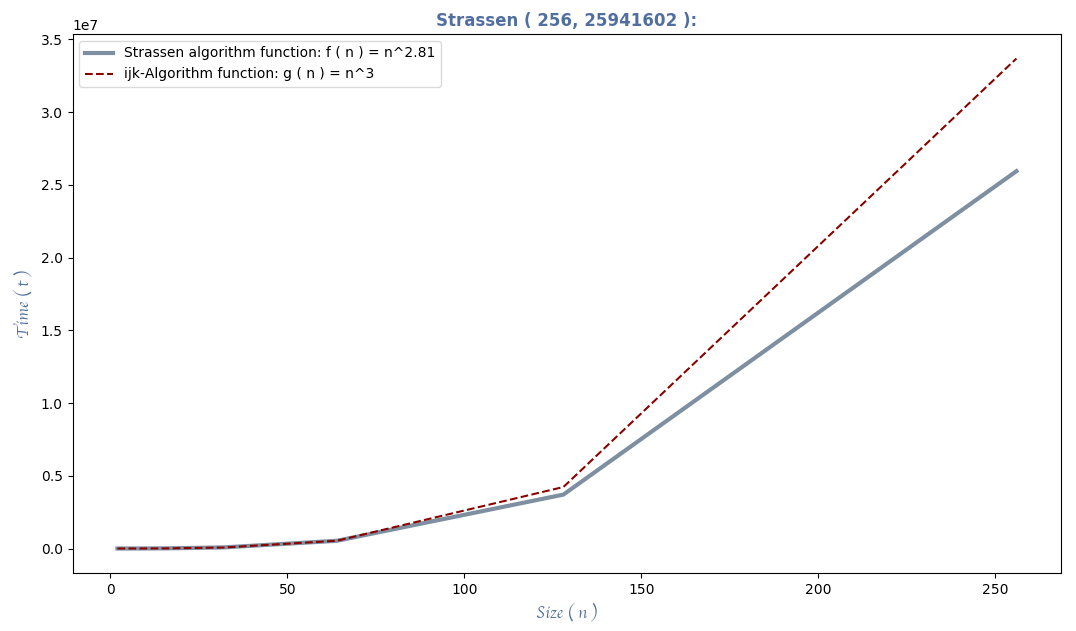
\includegraphics[width = 17cm, height = 10cm]{vg1.png}
\centering \linebreak \linebreak Figure 4.2.1: Graph for Figure 4.2.0.
\end{figure} \hfill

\begin{center}
\begin{tabular}[.5cm]{ c c c }
\toprule
Size ( $2^{n}$ ) & Strassen's Algorithm Time ( t ) & IJK-Algorithm Time ( t ) \\
\midrule
2 & 29 & 33 \\
\cmidrule {1-3}
4 & 218 & 173 \\
\cmidrule {1-3}
8 & 1541 & 1173 \\
\cmidrule {1-3}
16 & 10802 & 8741 \\
\cmidrule {1-3}
32 & 75629 & 67653 \\
\cmidrule {1-3}
64 & 529418 & 532613 \\
\cmidrule {1-3}
128 & 3705941 & 4227333 \\
\cmidrule {1-3}
 256 & 25941602 & 33686021 \\
\bottomrule
\linebreak
\end{tabular}
\linebreak \linebreak Table 3: Plot point for Strassen's and IJK Algorithms complexity of Figure 4.2.1.
\end{center}

\pagebreak

Second versus of {\bfseries\itshape Strassen's Algorithm} against {\bfseries\itshape IJK-Algorithm}. The program will plot the {\bfseries\itshape time} that both algorithm's takes to make the product of matrices of size {\itshape  n = $2^{9}$}. \hfill \break

\begin{figure}[H]
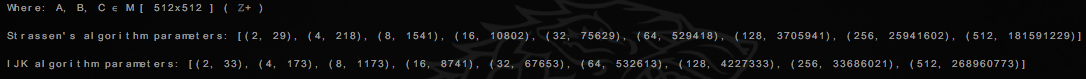
\includegraphics[width = 16.5cm, height = 1.5cm]{v2.png}
\centering \linebreak \linebreak Figure 4.2.2: Parameters of Strassen's and IJK algorithms for matrices of size n = $2^{9}$.
\end{figure} 

\begin{figure}[H]
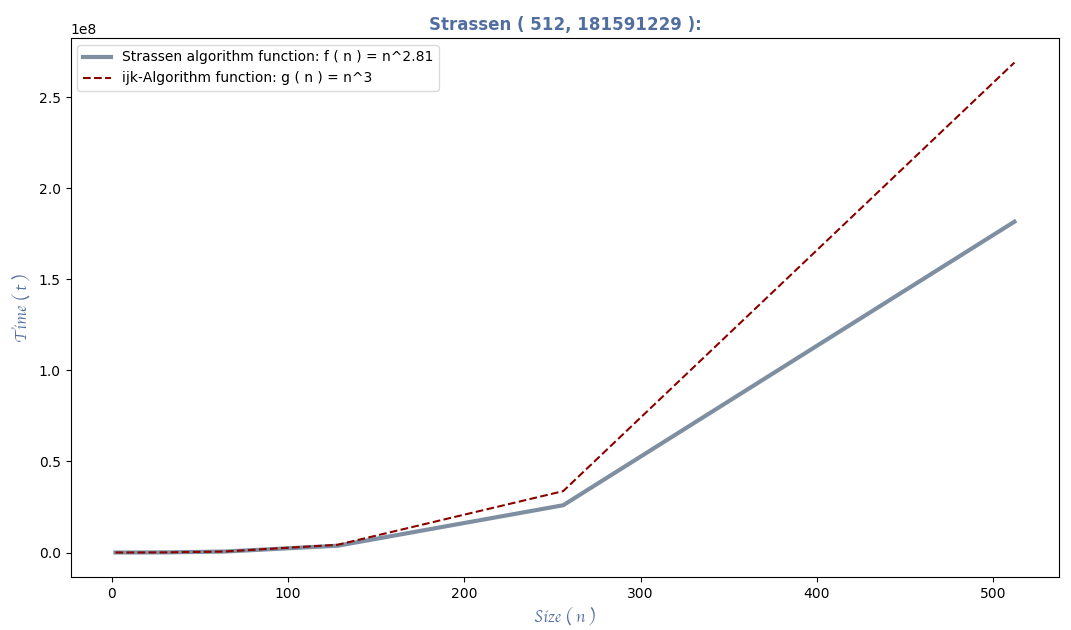
\includegraphics[width = 17cm, height = 10cm]{vg2.png}
\centering \linebreak \linebreak Figure 4.2.3: Graph for Figure 4.2.2.
\end{figure} \hfill

\begin{center}
\begin{tabular}[.5cm]{ c c c }
\toprule
Size ( $2^{n}$ ) & Strassen's Algorithm Time ( t ) & IJK-Algorithm Time ( t ) \\
\midrule
2 & 29 & 33 \\
\cmidrule {1-3}
4 & 218 & 173 \\
\cmidrule {1-3}
8 & 1541 & 1173 \\
\cmidrule {1-3}
16 & 10802 & 8741 \\
\cmidrule {1-3}
32 & 75629 & 67653 \\
\cmidrule {1-3}
64 & 529418 & 532613 \\
\cmidrule {1-3}
128 & 3705941 & 4227333 \\
\cmidrule {1-3}
 256 & 25941602 & 33686021 \\
 \cmidrule {1-3}
 512 & 181591229 & 268960773 \\
\bottomrule
\linebreak
\end{tabular}
\linebreak \linebreak Table 4: Plot point for Strassen's and IJK Algorithms complexity of Figure 4.2.3.
\end{center} \hfill

{\bfseries\itshape\color{carmine}{Observation:}} {\itshape\color{carmine}{The red function it's the IJK-Algorithm complexity: g ( n ) = $n^{3}$ and the blue it's the Stranssen's Algorithm complexity: f ( n ) = $n^{2.81}$.}} \hfill \break

\pagebreak